\chapter{Clojure.spec Study}

\section{Research questions}

I aim to answer these research questions:

\begin{itemize}
  \item What does the frequency and applications of \texttt{fdef} and \texttt{fspec} specs
    in open source software reveal about the utility of \texttt{clojure.spec}'s
    function semantics in practice?
\end{itemize}

I do not attempt to answer the following questions:

\begin{itemize}
  \item How frequently do users instrument specs for runtime verification?
\end{itemize}

\section{Methodology}

\subsection{Sources}

To determine the frequency of \texttt{fdef} and \texttt{fspec} specs,
the search features of \texttt{GitHub}~\footnote{\texttt{https://github.com}} and 
\texttt{CrossClj}~\footnote{\texttt{https://crossclj.info}} were used.

GitHub indexes tens of thousands of open source Clojure projects, and provides
a rudimentary search interface that is sufficient for discovering textual occurrences 
of functions and macros. False positives are common however, such as
GitHub does not distinguish
between ``toy'' projects and those with official releases, so we remove the former manually.
This is because toy projects do not give a good indication of real-world idioms---for example,
hundreds of projects simply contain experiments with \texttt{clojure.spec} that
are not officially released or maintained.

CrossClj maintains a rich database of cross-links between Clojure projects.
As of Febuary 2018, it indexes 9,438 projects, all of which have official releases (unlike
GitHub search) and thus have more credibility that they are used.
Cross-links are gathered for function/macro usages, and transitive project dependencies.
Unlike GitHub, CrossClj also distinguishes between ClojureScript and Clojure code

\subsection{Frequency Data gathering}

Simple GitHub searches were used to find occurrences of \texttt{fdef} and \texttt{fspec}.
As of March 2018,
searches for \texttt{fdef}
yield around 2,000 results~\footnote{\texttt{https://github.com/search?q=fdef+language\%3Aclojure\&type=Code}},
and for \texttt{fspec} 
\footnote{\texttt{https://github.com/search?q=fspec+language\%3Aclojure\&type=Code}}
yield around 600 results.
Searches were quite noisy, so less actual examples of these forms were found.

As a baseline, we searched for several common spec forms.
The spec \texttt{def} form for defining spec aliases found around 4,400 results.
The spec \texttt{keys} form for heterogeneous maps found around 3,500 results.
All of these numbers are compared in Figure~\ref{frequencybargraphs}.

CrossClj function/macro cross-links were used to find occurrences of spec idioms.
From the latest index (updated February 20th 2018)
\texttt{fdef} occurs in 721 top-level forms over 83 
projects~\footnote{\texttt{https://crossclj.info/fun/clojure.spec.alpha/fdef.html}}, and
\texttt{fspec} occurs in 22 top-level forms over 8 
projects~\footnote{\texttt{https://crossclj.info/fun/clojure.spec.alpha/fspec.html}}
(the mode number of occurrences per project was 1).

An error was found in the CrossClj data, however.
To find a baseline number of projects using \texttt{clojure.spec}, we looked for occurrences of
\texttt{s/def}, used to define spec
aliases. It should greatly outnumber the number of \texttt{fdef}'s in the ecosystem---we were
surprised to find CrossClj reports the opposite, and
we are almost certain these particular CrossClj metrics are incorrect.
We identified that multiple occurrences of \texttt{s/def} in the same project are not always counted by CrossClj,
so while CrossClj claims \texttt{s/def} occurs in more 60\% more projects than \texttt{fdef} (125), 
CrossClj reports \texttt{s/def} only occurs in 349 top-level 
forms~\footnote{\texttt{https://crossclj.info/fun/clojure.spec.alpha/def.html}}.
The latter number is too low---CrossClj reports, for example, the \texttt{clj-time}
library only has 2 occurrences of \texttt{s/def}, but it actually has 7 occurrences.

\begin{figure}
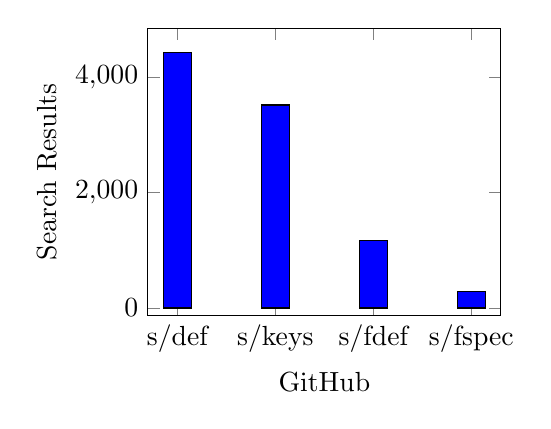
\begin{tikzpicture}
\begin{axis}[
  width=0.5\textwidth,
  symbolic x coords={s/def,s/keys,s/fdef,s/fspec},
    ylabel=Search Results,
    xlabel=GitHub,
    xtick=data]
    \addplot[ybar,fill=blue] coordinates {
         (s/def,4439)
         (s/keys,3522)
         (s/fdef,1167)
         (s/fspec,286)
                   };
\end{axis}
\end{tikzpicture}
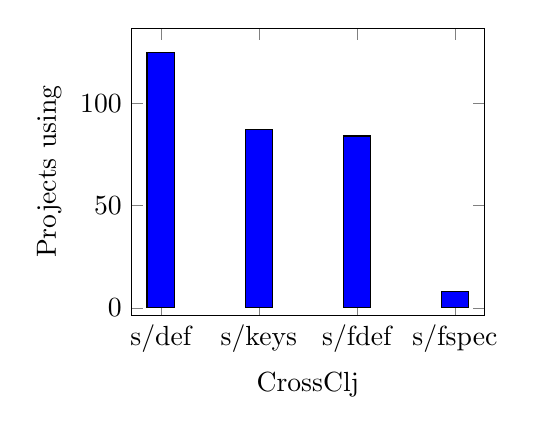
\begin{tikzpicture}
\begin{axis}[
  width=0.5\textwidth,
    symbolic x coords={s/def,s/keys,s/fdef,s/fspec},
    ylabel=Projects using,
    xlabel=CrossClj,
    xtick=data]
    \addplot[ybar,fill=blue] coordinates {
         (s/def,125)
         (s/keys,87)
         (s/fdef,84)
         (s/fspec,8)
                   };
\end{axis}
\end{tikzpicture}
\caption{Left, the number of results for GitHub searches about spec forms.
Right, the number of projects on CrossClj that use spec features.
  Searches for \texttt{ifn?} are omitted because
  it has been used as a common predicate since before 2009 (spec was released in 2017).
  }
  \label{frequencybargraphs}
\end{figure}

We did not notice such an error in the counts for \texttt{fspec} and \texttt{fdef}, but
this error reduces confidence on the exact numbers. Interestingly, the \emph{relative}
numbers of projects using these forms matches our intuition---\texttt{fspec} occurs
10 times less often than \texttt{fdef}, and \texttt{fdef} occurs about half as often as \texttt{s/def}
(see plot in Figure~\ref{frequencybargraphs}).
Still, these numbers should be treated with suspicion.

\subsection{Project Samples}

We selected 18 open source projects that use \texttt{fspec} to manually examine.
They were chosen by first searching GitHub for \texttt{fspec} occurrences, and
manually choosing the first few dozen results, manually keeping only projects
seemed to have official releases.
Figure~\ref{fspectable} summarizes these findings. We have included the project
names and our scratch notes as Appendix~\ref{appendix1}.

We also searched for negative examples of \texttt{fspec} usage---that is, occurrences
of higher-order functions with specs that did not use \texttt{fspec}---by searching for
both \texttt{fdef} and 
\texttt{ifn?}~\footnote{\texttt{https://github.com/search?utf8=\%E2\%9C\%93\&q=ifn\%3F+fdef+language\%3Aclojure\&type=Code}}, 
the flat contract for Clojure functions.
We selected 17 projects using a similar method via a GitHub search.
Appendix~\ref{appendix2} contains the projects and our scratch notes for this experiment.

\section{Experiment 1: Frequency of \texttt{fspec}}
\label{experiment1}

\begin{figure*}[t]

\begin{tabular}{lll}
      \toprule
  & \texttt{fspec} & \texttt{ifn?} \\
  \midrule
  Total occurrences in \texttt{fdef} & 79 & 3 \\
  \tabitem
  Total occurrences in \texttt{fdef} arguments & 65 (82\%) & 3 \\
  \tabitem
  Total occurrences in \texttt{fdef} return & 14  (18\%) & 0 \\
  Total occurrences in map spec & 41 & 2 \\
  \tabitem
  Total occurrences in heterogeneous map spec & 40 (97\%) & 2 \\
  \tabitem
  Total occurrences in homogeneous map spec & 1 (3\%) & 0 \\

\end{tabular}
\caption{Function specs in practice, in 18 open source projects sourced from GitHub that utilized \texttt{fspec}. }
\label{fspectable}
\end{figure*}

Our first investigation concentrated on projects that use \texttt{fspec}.
We chose 18 open source projects and manually investigated their usage of spec.

To gauge how \texttt{fspec}s are used in practice, we divided their occurrences
into several categories. 
Figure~\ref{fspectable} presents the results.

First, we measure how many times \texttt{fspec} occurs in top-level function
specs (i.e., \texttt{fdef} forms). Because spec has different semantics for
checking the argument and return of top-level function specs, we split this
category into occurrences in the arguments spec and return spec.
We also similarly measure the occurrences of \texttt{ifn?} in these projects,
which was sparsely used in these projects.

We found 82\% \texttt{fspec} instances occuring in the argument position,
with 18\% in the return position.

Second, we measure the frequency of \texttt{fspec} in a hash-map spec.
Of the occurrences of \texttt{fspec} in map specifications, 
we found a strong preference for using heterogeneous map specs (97\%),
with the rest being homogeneous maps.
If \texttt{fspec} occurs in a nested map, each map spec occurrence is counted.
Similar to the previous experiment, the flat function contract \texttt{ifn?} was rarely used 
in map specs in these projects.

We noticed several interesting things while conducting these experiments.

There was only 2 occurrence of nesting function specs more than 2 deep---in a library
that provides functional lenses~\footnote{https://github.com/andrewmcveigh/bifocal}.
Of those, one used 3 \texttt{fspec}s, the other 2 \texttt{fspec}s with a terminating \texttt{ifn?}.

We also noticed several users combining \texttt{fspec}s with the \texttt{or} spec
for disjunctions. It's unclear how well this works in practice (and might only be
there for documentation), but the ``looser'' generative testing semantics of \texttt{fspec}
seems to have more compatibility with disjunction contracts than the ``stricter''
proxy-based verification approach.

Spec also provides the ability to write dependent function contracts via the \texttt{:fn}
keyword option of \texttt{fspec}, allowing programmers
to add custom code to verify the relationship between function arguments and return values.
We found several interesting dependent contracts that used surprising techniques like
memoization to verify calls to higher-order functions~\footnote{https://github.com/CharlesHD/chu.graph}.

Some developers explicitly worked around the \texttt{fspec}'s generative testing semantics.
We found several comments and workarounds explaining why \texttt{fspec}s were not
appropriate in particular contexts. Common concerns were
\\
\begin{itemize}
	\item triggering function side effects,
	\item difficultly writing generators for testing the function, and
	\item being unsure whether generative testing was appropriate.
\end{itemize}

We speculate the lack of polymorphic function specs contributed to these concerns.
Since instances of a type variable were replaced with \texttt{any?} specs, writing
a generator often did not make sense. It's unclear whether polymorphic specs are
even feasible to check, but some developers at least seem attached to the documentation
capabilities of \texttt{fspec}, perhaps suggesting more control over the testing
semantics of \texttt{fspec} would be welcomed by spec users.

% function nesting:
% - lens library had largest nesting
% - depth 3 fspec's
% - depth 2 fspec's + terminating ifn?

\section{Experiment 2: Frequency of \texttt{ifn?}}
\label{experiment2}

\begin{figure*}[t]

\begin{tabular}{lll}
      \toprule
  & \texttt{fspec} & \texttt{ifn?} \\
  \midrule
  Total occurrences in \texttt{fdef} & 0 & 188 \\
  \tabitem
  Total occurrences in \texttt{fdef} arguments & 0 & 170 (90\%)\\
  \tabitem
  Total occurrences in \texttt{fdef} return & 0 & 18 (10\%)\\
  Total occurrences in map spec & 0 & 173 \\
  \tabitem
  Total occurrences in heterogeneous map spec & 0 & 67 (39\%) \\
  \tabitem
  Total occurrences in homogeneous map spec & 0 & 106 (61\%)\\

\end{tabular}
\caption{Flat function specs in practice, in 17 open source projects sourced from GitHub that utilized \texttt{ifn?}.
The 106 homogeneous map spec occurrences were sourced from only 3 of the projects, one project contributing the maximum 93 occurrences.
Heterogeneous map specs occurrences were from 7 of the projects, with maximum 30 occurrences in one project.
}
\label{ifntable}
\end{figure*}

In our second experiment, we measured the frequency of \texttt{ifn?} in 17 open source projects.
The results are summarised in Figure~\ref{ifntable}.

Similar to our first experiment, occurrences of \texttt{ifn?} were mostly in the argument
positions in \texttt{fdef} (90\%).
The data for \texttt{ifn?} occurrences in map specs is somewhat skewed, since one project
contributed over half of the occurrences. However, even without taking that project into account,
around half of all the \texttt{ifn?} occurrences were found in map specs.

One striking divide we noticed was the obvious preference for either \texttt{ifn?} or \texttt{fspec}
per project. None of the projects that primarily used \texttt{ifn?} used \texttt{fspec} even once.
In the first experiment, projects that used \texttt{fspec} used \texttt{ifn?} rarely---mostly to
avoid \texttt{fspec}'s generative testing semantics.

\section{Conclusions}

Our goal in this section was to inform our decisions for when to generate \texttt{fspec}
annotations in our automatic spec annotation tool.
We surveyed open source projects via GitHub by measuring instances of two kinds of projects:
those that primarily used \texttt{fspec}, and those that primarily used \texttt{ifn?}.

Our experiments yielded many interesting insights. Even using broad measurements like
GitHub searches and CrossClj project references,
we consistently found other common spec features were used roughly an order of
magitude more than \texttt{fspec} (Figure~\ref{frequencybargraphs}).

However, we still investigated how programmers use \texttt{fspec} (Section~\ref{experiment1}).
In the projects that primarily used \texttt{fspec} for first-class function specs,
we found several instances of programmers enjoying the expressive documentation
of \texttt{fspec}, but avoiding its generative testing semantics in creative ways.
Sometimes \texttt{fspec}s commented out and replaced with \texttt{ifn?}, implying
spec might benefit from more control over \texttt{fspec}'s testing semantics.

Our second experiment (Section~\ref{experiment2}) measured how programmers combined
spec with \texttt{ifn?}.
Interestingly, none of the 17 projects we selected used \texttt{fspec}---programmers
seem divided in strong preferences for \texttt{ifn?} and \texttt{fspec}, with
\texttt{fspec} users using \texttt{ifn?} only occasionally to work around
\texttt{fspec}'s testing semantics.

A unique feature of spec's runtime instrumentation of \texttt{fdef}s is that
return values are not checked. Since we predicted programmers might have
issues with \texttt{fspec}'s generative testing semantics, we were interested
if \texttt{fspec}'s were more frequent than usual in the return position
of \texttt{fdef} (where these semantics would be implicitly suppressed).
In our investigation, we found no particular evidence that programmers preferred
\texttt{fspec} over \texttt{ifn?} in the return position---when they occurred in \texttt{fdef} forms,
\texttt{fspec} was in the return position 18\% of the time (Figure~\ref{fspectable}),
and \texttt{ifn?} was 10\% of the time (Figure~\ref{ifntable}).

One difference we found was \texttt{ifn?} occurs with a high correlation in
a map spec (92\% of the time), while \texttt{fspec} occurred in a map spec
only 51\% of the time.
However, \texttt{fspec} occurred much more often in heterogeneous map specs
(97\% of occurrences in map specs were heterogeneous), while \texttt{ifn?}
only occurred in heterogeneous maps 39\% of the time.
Heterogeneous maps in Clojure are used like records or structs in other
languages~\cite{bonnaire2016practical}, so the appeal of combining
\texttt{fspec} with heterogeneous maps is similar to giving precise annotations
to record or struct fields.

The lack of polymorphism in spec coupled with the frequency of polymorphic functions
in Clojure seems to be a strong reason to prefer \texttt{ifn?} in many situations.
We found \texttt{ifn?} was often used to avoid ``any to any'' function
specs, which would otherwise use the generator for \texttt{any?} to generatively test
the function value. This is inappropriate for many common variants on polymorphic functions like
\texttt{map}, \texttt{filter}, and \texttt{reduce}
and we found several examples in our experiments that support this view
(see occurrences of ``polymorphic'' in Appendix~\ref{appendix2}).

% how does no polymorphism interact with fspec semantics? are they more useful together?

To tie back our investigation---what does this tell us about programmer preferences in an automatic spec annotation
tool? At the very least, it tells us there is no simple ``fits all'' behavior---we found
preferences were in (at least) two distinct camps.
This implies that the tool should have some customizability between preferring
\texttt{fspec} and \texttt{ifn?}, but which should be the default?

Should the tool prefer more expressive, but possibly incorrect specs, over less
expressive but specs that ``just work''?
I don't think there is a single definitive answer---rather each occurrence of \texttt{fspec}
comes with its own context and tradeoffs. Whether it occurs in the arguments or return of
an \texttt{fdef}, in a heterogeneous or homogeneous map, or even nested in another \texttt{fspec}
are relevant contextual information that the default behavior of the tool should take
into account. The varied and subtle results of this investigation support the conclusion
that the tool's behavior should probably itself be varied and subtle.

